\documentclass{article}

\usepackage[hmargin=1in, vmargin=.75in]{geometry}
\usepackage[citecolor=blue, colorlinks=true, linkcolor=blue, urlcolor=blue]{hyperref}
\usepackage{natbib}
\usepackage{graphicx}
\usepackage{authblk}

\title{MT Metadata Guide}
\author[1]{IRIS-PASSCAL MT Software Development Committee}
\affil[1]{IRIS}

\newcommand{\attr}[1]{\textbf{#1}}
\renewcommand{\arraystretch}{1.35}

\begin{document}
	
\maketitle

\tableofcontents

\newpage

\section{Introduction}

The magnetotelluric community is relatively small which has led to various formats for storing the time series data.  Some type of ASCII format seems to be the most prevalent because before large data sets that was the easiest method of storage. Various binary formats exist, some proprietary and some open like the Scripps format, though efficient, these files lack some critical metadata.  Metadata is key to archiving data and as of now there has been no documentation on metadata standards for MT time series data.  

IRIS-PASSCAL is adding MT capabilities to their instrument pool and has setup a committee to develop MT metadata standards for archiving time series.  What follows are the metadata standards developed by that committee.


\section{General Structure}

The MT metadata standards are structured to cover details from single channel time series to the full MT survey.  For simplicity each of the different scales of an MT survey and measurements have been categorized starting from largest scale to smallest scale (Figure \ref{fig:example}).  These categories are: \verb|Survey|, \verb|Station|, \verb|Run|, \verb|DataLogger|, \verb|Channel| which has different attributes depending on what type of channel it is, magnetic, electric, auxiliary.  Each of these will be described in the sections below.  

\begin{figure}[htb!]
	\centering
	\includegraphics[height=.625\textheight]{example_mt_file_structure.pdf}
	\caption{Schematic of a MT time series file structure with appropriate metadata.}
	\label{fig:example}
\end{figure}

\subsection{Metadata Keyword Format}

The metadata key names should be self explanatory and they are structured as follows: \verb|name_type| or \verb|category/name_type|, where \verb|name| is the description name, \verb|type| is the data type (Table \ref{tab:types}), and \verb|category| refers to a metadata category that has common parameters, such as \verb|location| which will have an x, y, and z $\longrightarrow$ \verb|location/x_d|, \verb|location/y_d|, and \verb|location/z_d|. This will help keep order and help users understand the metadata without having to consult the documentation all the time. 

\begin{table}[htb!]
	\caption[Data types]{Permissible values for data types}
	\begin{tabular}{|l|l|}
		\hline
		\textbf{Data Type} & \textbf{Label} \\
		\hline
		String & s \\ \hline
		Double (float) & d \\ \hline
		Integer & i \\ \hline
		Boolean & b \\ \hline
	\end{tabular}
	\label{tab:types}
\end{table}

\subsection{Formatting Standards}

There are certain formatting standards that need to be adhered to, specifically location, time and date, and angles.

\subsubsection{Time and Date Format}

All time and dates are given as an ISO formatted date-time string in the UTC time zone.  The ISO date time format is \verb|YYYY-MM-DDThh:mm:ss.ms+00:00|.  Milliseconds can be accurate to 6 decimal places.  Dates are formatted \verb|YYYY-MM-DD|.  Other formats can be input but only ISO format will be output.  Internally, all date time strings are converted to a \verb|datetime| object which can output various formats like epoch seconds, which will keep date-times self consistent.

\subsubsection{Location}

All latitude and longitude locations are given in decimal degrees. Other formats can be input but will only be output as decimal degrees.

\begin{itemize}
	\setlength\itemsep{0em}
	\item All latitude values must be $<|90|$ and all longitude values must be $<|180|$.
	\item Elevation and other distance values are given in meters.
	\item Datum should be one of the well known datums, WGS84 is preferred, but others are acceptable.
\end{itemize} 

\textbf{Note:} The one exception is sensor location which can be in units relative to the station location?  

\subsubsection{Angles}

All angles of orientation are given in degrees.  Orientation of dipoles and magnetometers are relative to \verb|station_orientation_s|.  Otherwise angles are assumed to be clockwise positive from Geographic North = 0.  

\newpage
\section{Survey}

A survey describes an entire MT survey that covers a specific study area.  This may include multiple researchers and research groups or a multi-year campaign, but should be confined to a specific regional area.  The \verb|Survey| metadata category describes the general parameters of the survey. 

\begin{table}[htb!]
	\caption[Attributes for Survey]{Attributes for Survey category}
	\begin{tabular}{|l|l|l|l|}
		\hline
		\textbf{Metadata Key} & \textbf{Description} & \textbf{Type} & \textbf{Required} \\ \hline
		name\_s & name of survey & string & compulsory \\ \hline
		id\_s & nickname of survey & string & optional \\ \hline
		net\_code\_s & network code given by IRIS & string & compulsory \\ \hline
		start\_date\_s & start date of survey [ UTC ] & string & compulsory \\ \hline
		end\_date\_s & end date of survey [ UTC ] & string & compulsory \\ \hline
		northwest\_corner/latitude\_d & location of northwest corner of survey [ degrees (hh.mmss) ] & float & compulsory \\ \hline
		northwest\_corner/longitude\_d & location of northwest corner of survey [ degrees (hh.mmss) ] & float & compulsory \\ \hline
		southeast\_corner/latitude\_d & location of southeast corner of survey  [ degrees (hh.mmss) ] & float & compulsory \\ \hline
		southeast\_corner/longitude\_d & location of southeast corner of survey  [ degrees (hh.mmss) ] & float & compulsory \\ \hline
		datum\_s & "datum of x and y coordinates [ WGS84 ]" & string & compulsory \\ \hline
		location\_s & location of survey in general terms & string & optional \\ \hline
		country\_s & country/countries survey located in & string & optional \\ \hline
		summary\_s & summary paragraph of survey & string & compulsory \\ \hline
		notes\_s & notes about survey & string & optional \\ \hline
		acquired\_by/author\_s & principal investigator(s) responsible for survey & string & compulsory \\ \hline
		acquired\_by/organization\_s & organization(s) associated with survey & string & compulsory \\ \hline
		acquired\_by/email\_s & email address of PI(s) & string & compulsory \\ \hline
		acquired\_by/url\_s & url(s) of organization(s) & string & compulsory \\ \hline
		release\_status\_s & release status [ open $|$ on request $|$ propriatary $|$...] & string & compulsory \\ \hline
		conditions\_of\_use\_s & condition of use information information including licensing & string & optional \\ \hline
		citation\_dataset/doi\_s & citation dataset doi number & string & compulsory \\ \hline
		citation\_journal/doi\_s & citation journal doi & string & optional \\ \hline
	\end{tabular}
	\label{tab:survey}
\end{table} 

\newpage
\subsection{Example Survey JSON String}

\begin{verbatim}
{
 "name_s": "Long Valley, CA",
 "id_s": "Casa Diablo",
 "net_code_s": "network code given by IRIS",
 "start_date_s": "2020-01-01",
 "end_date_s": "2021-01-01",
 "northwest_corner/latitude_d": 37.5,
 "northwest_corner/longitude_d": 122,
 "southeast_corner/latitude_d": 36.5,
 "southeast_corner/longitude_d": -121.15,
 "datum_s": "WGS84",
 "location_s": "Mammoth, CA",
 "country_s": "USA",
 "summary_s": "This survey is meant to image the magmatic and hydrothermal systems.",
 "notes_s": "Had complications due to snow",
 "acquired_by/author_s": "M. Tee, T. Luric, S. Spot, and A. Borealis",
 "acquired_by/organization_s": "MT Gurus",
 "acquired_by/email_s": "mtee@guru.com",
 "acquired_by/url_s": "mt_guru.com",
 "release_status_s": "open",
 "conditions_of_use_s": "condition of use information information including licensing",
 "citation_dataset/doi_s": "citation dataset doi number",
 "citation_journal/doi_s": "citation journal doi",
}
\end{verbatim}

\newpage
\section{Station}

A station is a single location where MT data are collected, if the location of the station is moved during a run, then a new station should be created. If the sensors, cables, data logger, battery were replaced during a run but the station remained at the same location, that can be recorded in the \verb|Run| metadata, but is still considered a station.

\begin{table}[htb!]
	\caption[Attributes for Station]{Attributes for Station category}
	\begin{tabular}{|l|p{3in}|l|l|}
		\hline
		\textbf{Metadata Key} & \textbf{Description} & \textbf{Type} & \textbf{Required} \\ \hline
		sta\_code\_s & 5 char name of station & string & compulsory \\ \hline
		name\_s & name station site & string & compulsory \\ \hline
		latitude\_d & longitude location [ degrees (hh.mmss) ] & float & compulsory \\ \hline
		longitude\_d & latitude location [ degrees (hh.mmss) ] & float & compulsory \\ \hline
		elevation\_d & elevation [ m ] & float & compulsory \\ \hline
		notes\_s & any notes about station & string & optional \\ \hline
		datum\_s & datum for lat, lon location & string & compulsory \\ \hline
		start\_s & start time and date of data logging [ UTC ] & string & compulsory \\ \hline
		end\_s & stop time and date of data logging  [ UTC ] & string & compulsory \\ \hline
		num\_channels\_i & number of channels recording & int & compulsory \\ \hline
		channels\_recorded\_s & "list of channels recorded [EX, EY, HX, HY, HZ $|$ ...]" & string & compulsory \\ \hline
		data\_type\_s & type of data collected [ BB $|$ LP $|$ AMT $|$ Combo $|$ ...] & string & compulsory \\ \hline
		declination/value\_d & declination value & float & compulsory \\ \hline
		declination/units\_s & declination units [ degrees ] & string & compulsory \\ \hline
		declination/epoch\_s & declination epoch & string & compulsory \\ \hline
		declination/model\_s & declination model & string & compulsory \\ \hline
		station\_orientation\_s & orientation coordinate system [ geographic $|$ channel-measurement specific ] & string & compulsory \\ \hline
		orientation\_method\_s & [ compass $|$ differential GPS $|$ gyroscope $|$...] & string & optional \\ \hline
		acquired\_by/author\_s & person(s) operating station & string & compulsory \\ \hline
		acquired\_by/email\_s & email of lead station operator & string & compulsory \\ \hline
		provenance/creation\_time\_s & creation time of time series data for storing & string & compulsory \\ \hline
		provenance/software/name\_s & name of software used to store time series & string & compulsory \\ \hline
		provenance/software/version\_s & version of software used to store time series & string & compulsory \\ \hline
		%		provenance/software/author\_s & author of software used to store time series & string & compulsory \\ \hline
		%		provenance/creator/author\_s & name of person or group creating archive data & string & compulsory \\ \hline
		%		provenance/creator/organization\_s & name of organization or institution creating archive data & string & compulsory \\ \hline
		%		provenance/creator/url\_s & url of group creating archive data & string & compulsory \\ \hline
		%		provenance/creator/email\_s & email of person or group creating archive data & string & compulsory \\ \hline
		provenance/submitter/author\_s & name of person or group submitting archive data & string & compulsory \\ \hline
		provenance/submitter/organization\_s & name of organization or institution submitting archive data & string & compulsory \\ \hline
		provenance/submitter/url\_s & url of group submitting archive data & string & compulsory \\ \hline
		provenance/submitter/email\_s & email of person or group submitting archive data & string & compulsory  \\ \hline
		provenance/notes\_s & any notes on the history of the data & string & optional \\ \hline
		provenance/log\_s & log of any changes made to time series data & string & optional \\ \hline
	\end{tabular}
\label{tab:station01}
\end{table}	
   
\newpage
\subsection{Example Station JSON String}

\begin{verbatim}
{
 "sta_code_s": "MNP01",
 "name_s": "Mojave National Preserve Hole-in-the-rock",
 "latitude_d": 35.0,
 "longitude_d": -117.0,
 "elevation_d": 1200,
 "notes_s": "Donkeys chewed both electric channels",
 "datum_s": "WGS84",
 "start_s": "2020-01-01T12:00:00.0000 UTC",
 "end_s": "2020-01-12T12:00:00.0000 UTC",
 "num_channels_i": 5,
 "channels_recorded_s": "[EX, EY, HX, HY, HZ]",
 "data_type_s": "BB & LP",
 "declination/value_d": "11.5",
 "declination/units_s": "degrees",
 "declination/epoch_s": "declination epoch",
 "declination/model_s": "WMM2019-2024",
 "station_orientation_s": "geographic",
 "orientation_method_s": "compass",
 "acquired_by/author_s": "M. Tee and A. Borealis",
 "acquired_by/email_s": "m.tee@guru.com",
 "provenance/creation_time_s": "2020-05-01T12:00:00.0000 UTC",
 "provenance/software/name_s": "MTH5",
 "provenance/software/version_s": "1.0.0",
 "provenance/software/author_s": "IRIS",
 "provenance/submitter/author_s": "M. Tee",
 "provenance/submitter/organization_s": "MT Gurus",
 "provenance/submitter/url_s": "mt_guru.com",
 "provenance/submitter/email_s": "m.tee@guru.com",
 "provenance/notes_s": "Electrics are good until 2020-01-10",
 "provenance/log_s": "The data was rotated using an updated declination 2020-05-02."
}
\end{verbatim}

\newpage
\section{Run}

A run is data collected at a single station at a single sampling rate.  If the dipole length or other such station parameters are changed between runs that is ok, just make a new run.  If the station is relocated then a new station should be created.

\begin{table}[htb!]
	\caption[Attributes for Run]{Attributes for Run category}
	\begin{tabular}{|l|p{3in}|l|l|}
		\hline
		\textbf{Metadata Key} & \textbf{Description} & \textbf{Type} & \textbf{Required} \\ \hline
		id\_s & run ID & string & compulsory \\ \hline
		notes\_s & notes on run & string & optional \\ \hline
		start\_s & start date and time of data logging [ UTC ] & string & compulsory \\ \hline
		end\_s & stop date and time of data logging [ UTC ] & string & compulsory \\ \hline
		sampling\_rate\_d & sampling rate of run (samples/second) & float & compulsory \\ \hline
		num\_channels\_i & number of channels recorded & int & compulsory \\ \hline
		channels\_recorded\_s & "list of channels recorded [ [EX, EY, HX, HY] $|$ ...]" & string & compulsory \\ \hline
		data\_type \_s & type of data collected [ BB $|$ LP $|$ AMT $|$ Combo $|$ ...] & string & compulsory \\ \hline
		acquired\_by/author\_s & person(s) responsible for run & string & compulsory \\ \hline
		acquired\_by/email\_s & email of lead run operator & string & compulsory \\ \hline
		provenance/notes\_s & any notes on the history of the data & string & optional \\ \hline
		provenance/log\_s & log of any changes made to time series data & string & optional \\ \hline
	\end{tabular}
	\label{tab:run}
\end{table}

\subsection{Example Run JSON String}

\begin{verbatim}
{
 "id_s": "MNP02_b",
 "notes_s": "Changed north electrode",
 "start_s": "2020-01-02T15:30:00.0000 UTC",
 "end_s": "2020-01-05T07:05:30.0000 UTC",
 "sampling_rate_d": 256,
 "num_channels_i": 5,
 "channels_recorded_s": "[EX, EY, HX, HY, HZ]",
 "data_type_s": "BB",
 "acquired_by/author_s": "T. Luric",
 "acquired_by/email_s": "t.lurric@guru.com",
 "provenance/notes_s": "Near a powerline and HZ is clipped",
 "provenance/log_s": "Clipped data in HZ replaced with zeros 2020-05-01 by T. Luric"
}
\end{verbatim}

\newpage
\section{Data Logger}

Data logger is a the digital acquisition system used to collect time series data at a single station for a single run.  \verb|DataLogger| metadata includes the type of data logger, timing system, firmware, number of channels, calibrations, and power source.

\begin{table}[htb!]
	\caption[Attributes for DataLogger]{Attributes for DataLogger category}
	\begin{tabular}{|l|p{3in}|l|l|}
		\hline
		\textbf{Metadata Key} & \textbf{Description} & \textbf{Type} & \textbf{Required} \\ \hline
		manufacturer\_s & manufacturer name & string & compulsory \\ \hline
		model\_s & model name & string & compulsory \\ \hline
		serial\_s & serial number & string & compulsory \\ \hline
		notes\_s & notes about data logger & string & compulsory \\ \hline
		timing\_system/type\_s & type of timing system [GPS $|$ internal $|$ ... ] & string & compulsory \\ \hline
		timing\_system/drift\_d & any drift in internal clock & float & compulsory \\ \hline
		timing\_system/uncertainty\_d & uncertainty associated with internal clock & float & compulsory \\ \hline
		timing\_system/notes\_s & notes on timing system & string & optional \\ \hline
		firmware/version\_s & firmware version & string & compulsory \\ \hline
		firmware/date\_s & date on firmware & string & compulsory \\ \hline
		firmware/author\_s & author of firmware & string & optional \\ \hline
		n\_channels\_i & number of channels & int & compulsory \\ \hline
		n\_channels\_used\_s & number of channels used & int & compulsory \\ \hline
		power\_source/type\_s & power source type [ Pb-acid battery $|$ solar panel $|$ Li battery $|$ ...] & string & compulsory \\ \hline
		power\_source/start\_voltage\_d & starting voltage of power source & float & compulsory \\ \hline
		power\_source/end\_voltage\_d & ending voltage of power source & float & compulsory \\ \hline
		power\_source/notes\_s & notes on power source & string & optional \\ \hline
	\end{tabular}
	\label{tab:datalogger}
\end{table}	

\newpage
\subsection{Example DataLogger JSON String}

\begin{verbatim}
{
 "manufacturer_s": "MT `r Us",
 "model_s": "Broadband 2000",
 "serial_s": "0128947850230",
 "notes_s": "Intern dropped the data logger on a shovel.",
 "timing_system/type_s": "GPS",
 "timing_system/drift_d": 0,
 "timing_system/uncertainty_d": .0000016,
 "timing_system/notes_s": "only works when sky is clear",
 "firmware/version_s": "1.0",
 "firmware/date_s": "2020-01-01",
 "firmware/author_s": "R. Phase",
 "n_channels_i": 5,
 "n_channels_used_s": 4,
 "power_source/type_s": "solar panel and battery]",
 "power_source/start_voltage_d": 13.1,
 "power_source/end_voltage_d": 12.0,
 "power_source/notes_s": "Overcast all day reduced recharging"
}
\end{verbatim}

\newpage
\section{Electric Channel}

Electric channel refers to a dipole measurement of the electric field for a single station for a single run.
 
\begin{table}[htb!]
	\caption[Attributes for Electric Channel]{Attributes for Electric category}
	\begin{tabular}{|l|p{3in}|l|l|}
		\hline
		\textbf{Metadata Key} & \textbf{Description} & \textbf{Type} & \textbf{Required} \\ \hline
		dipole/length\_d & length of dipole [ m ] & float & compulsory \\ \hline
		channel\_num\_i & channel number [ 1 $|$ 2 $|$ 3 $|$ 4 $|$ 5 $|$ 6 $|$...] & int & compulsory \\ \hline
		component\_s & [ Ex $|$ Ey $|$ Ez ] & string  & compulsory \\ \hline
		azimuth\_d & azimuth of dipole N = 0,  E = 90 [ degrees ] & float & compulsory \\ \hline
		positive/ID\_s & sensor id number & string & compulsory \\ \hline
		positive/latitude\_d & positive sensor location latitude [ degrees (hh.mmss) ] & float & optional \\ \hline
		positive/longitude\_d & positive sensor location longitude [ degrees (hh.mmss) ] & float & optional \\ \hline
		positive/elevation\_d & positive sensor location elevation [ m ] & float & optional \\ \hline
		positive/datum\_s & "positive datum for x, y, z location [ WGS84 ]" & string & optional \\ \hline
		positive/sensor\_type\_s & type of electric sensor [ Ag-AgCl $|$ Pb-PbCl $|$ ...] & string & compulsory \\ \hline
		positive/sensor\_manufacturer\_s & electric sensor manufacturer & string & compulsory \\ \hline
		positive/sensor\_notes\_s & notes on electric sensor & string & optional \\ \hline
		negative/ID\_s & sensor id number & string & compulsory \\ \hline
		negative/longitude\_d & negative sensor location latitude [ degrees (hh.mmss) ] & float & optional \\ \hline
		negative/latitude\_d & negative sensor location longitude [ degrees (hh.mmss) ] & float & optional \\ \hline
		negative/elevation\_d & negative sensor location elevation [ m ] & float & optional \\ \hline
		negative/datum\_s & "negative datum for x, y, z location [ WGS84 ]" & string & optional \\ \hline
		negative/sensor\_type\_s & type of electric sensor [ Ag-AgCl $|$ Pb-PbCl $|$ ...] & string & compulsory \\ \hline
		negative/sensor\_manufacturer\_s & electric sensor manufacturer & string & compulsory \\ \hline
		negative/sensor\_notes\_s & notes on electric sensor & string & optional \\ \hline
		contact\_resistance/start\_A\_d & contact resistance at beginning of measurement, positive polarity [ Ohm ]" & float & optional \\ \hline
		contact\_resistance/start\_B\_d & contact resistance at beginning of measurement, negative polarity [ Ohm ] & float & optional \\ \hline
		contact\_resistance/end\_A\_d & contact resistance at end of measurement, positive polarity [ Ohm ] & float & optional \\ \hline
		contact\_resistance/end\_B\_d & contact resistance at end of measurement, negative polarity [ Ohm ] & float & optional \\ \hline
		ac/start\_d & AC at start of measurement [ V ] & float & optional \\ \hline
		ac/end\_d & AC at end of measurement [ V ] & float & optional \\ \hline
		dc/start\_d & DC at start of measurement [ V ] & float & optional \\ \hline
		dc/end\_d & DC at end of measurement [ V ] & float & optional \\ \hline
		
	\end{tabular}
	\label{tab:electric01}
\end{table}	

\newpage
\begin{table}[htb!]
	\caption[Attributes for Electric Channel cont`d]{Attributes for Electric category continued}
	\begin{tabular}{|l|p{3in}|l|l|}
		\hline
		\textbf{Metadata Key} & \textbf{Description} & \textbf{Type} & \textbf{Required} \\ \hline
		units\_s & units of electric field data [ counts $|$ mV/km $|$ ... ] & string & compulsory \\ \hline
		sample\_rate\_d & sample rate of electric channel (samples/second) & float & compulsory \\ \hline
		notes\_s & notes about electric field measurement & string &  optional \\ \hline
		data\_quality/rating\_d & data quality rating based on some sort of statistic & float & optional \\ \hline
		data\_quality/warning\_comments\_s & any warnings about data quality & string & optional \\ \hline
		data\_quality/warning\_flags\_d & a value flagging bad data  & float &  optional \\ \hline
		data\_quality/author\_s & person who did QC/QA on data & string &  optional \\ \hline
		filter/name\_s & filter name in filter table, can be a list. Needs to be ordered in which filters were applied & string &  optional \\ \hline
		filter/notes\_s & any notes on the filtering & string &  optional \\ \hline
		filter/applied\_b & have filters been applied [ True $|$ False ] & string & compulsory \\ \hline
		\end{tabular}
		\label{tab:electric02}
\end{table}	

\newpage
\subsection{Example Electric Channel JSON String}

\begin{verbatim}
{
 "dipole/length_d": 59.7,
 "channel_num_i": 1",
 "component_s": EX,
 "azimuth/value_d": 0,
 "positive/id_s": "101",
 "positive/latitude_d": 35.5578,
 "positive/longitude_d": -117.38754,
 "positive/elevation_d": 103.4,
 "positive/datum_s": "WGS84",
 "positive/sensor_type_s": "Ag-AgCl"
 "positive/sensor_manufacturer_s": "Zaps",
 "positive/sensor_notes_s": "Sitting on the shelf since last year",
 "negative/id_s": "102",
 "negative/latitude_d": 35.5588,
 "negative/longitude_d": -117.38754,
 "negative/elevation_d": 105.8,
 "negative/datum_s": "WGS84",
 "negative/sensor_type_s": "Ag-AgCl"
 "negative/sensor_manufacturer_s": "Zaps",
 "negative/sensor_notes_s": "Sitting on the shelf since last year",
 "contact_resistance/start_A_d": 1200.0,
 "contact_resistance/start_B_d": 1210.0,
 "contact_resistance/end_A_d": 1205.0,
 "contact_resistance/end_B_d": 1205.0,
 "ac/start_d": 0.03,
 "ac/end_d": 0.04,
 "dc/start_d": 0.001,
 "dc/end_d": 0.002,
 "units_s": "counts",
 "sample_rate_d": 256,
 "notes_s": "cables chewed on 2020-01-07",
 "data_quality/rating_d": 3,
 "data_quality/warning_comments_s": "cables chewed 2020-01-07",
 "data_quality/warning_flags_s": "Nan",
 "data_quality/author_s": "Q. Sea",
 "filter/name_s": "[counts2mv, datalogger024]",
 "filter/notes_s": "notes on filters applied",
 "filter/applied_b": "True"
}
\end{verbatim}

\newpage
\section{Magnetic Channel}

A magnetic channel is a recording of one component of the magnetic field at a single station for a single run.

\begin{table}[htb!]
	\caption[Attributes for Magnetic Channel]{Attributes for Magnetic category}
	\begin{tabular}{|l|p{3in}|l|l|}
		\hline
		\textbf{Metadata Key} & \textbf{Description} & \textbf{Type} & \textbf{Required} \\ \hline
		sensor/type\_s & type of magnetic sensor [ Induction Coil $|$ flux gate $|$ ...] & string & compulsory \\ \hline
		sensor/manufacturer\_s & magnetic sensor manufacturer & string &  compulsory \\ \hline
		sensor/notes\_s & notes on sensor & string & compulsory \\ \hline
		sensor/ID\_s & sensor id number & string &  compulsory \\ \hline
		channel\_num\_i & channel number [ 1 $|$ 2 $|$ 3 $|$ 4 $|$ 5 $|$ 6 $|$...] & int &  compulsory \\ \hline
		component\_s & [ Hx $|$ Hy $|$ Hz ] & string  &  compulsory \\ \hline
		azimuth\_d & azimuth in \verb|station\_coordinates_s| [ degrees ]& float & compulsory \\ \hline
		longitude\_d & sensor longitude degrees & float & compulsory \\ \hline
		latitude\_d & sensor latitude in degrees & float &  compulsory \\ \hline
		elevation\_d & sensor elevation in meters & float &  compulsory \\ \hline
		datum\_s & datum for location [ WGS84 $|$ ... ] & string &  compulsory\\ \hline
		units\_s & units of magnetic field data [ counts $|$ mV $|$ ... ] & string &  compulsory \\ \hline
		sample\_rate\_d & sample rate of magnetic channel (samples/second) & float &  compulsory \\ \hline
		h\_field/min\_start\_d & minimum h-field value at beginning of measurement & float &  optional \\ \hline
		h\_field/max\_start\_d & maximum h-field value at beginning of measurement & float &  optional\\ \hline
		h\_field/min\_end\_d & minimum h-field value at end of measurement & float &  optional\\ \hline
		h\_field/max\_end\_d & maximum h-field value at end of measurement & float &  optional\\ \hline
		h\_field/units\_s & units of h-field measurement [ nT $|$ ...] & string &   optional \\ \hline
		notes\_s & notes on magnetic field measurments & string &  optional \\ \hline
		data\_quality/rating\_d & data quality rating based on some sort of statistic & float &  optional \\ \hline
		data\_quality/warning\_comments\_s & any warnings about data quality & string &   optional \\ \hline
		data\_quality/warning\_flags\_s & a value flagging bad data  & float &  optional \\ \hline
		data\_quality/author\_s & person who did QC/QA on data & string &   optional \\ \hline
		filter/name\_s & filter name in filter table, can be a list. Needs to be ordered in which filters were applied & string &  optional \\ \hline
		filter/notes\_s & any notes on the filtering & string &  optional \\ \hline
		filter/applied\_b & have filters been applied [ True $|$ False ] & string & compulsory \\ \hline
		\end{tabular}
	\label{tab:magnetic}
\end{table}

\newpage
\subsection{Example Magnetic Channel JSON String}

\begin{verbatim}
{
 "sensor/type_s": "Induction Coil",
 "sensor/manufacturer_s": "MT `r Us",
 "sensor/notes_s": "new coil",
 "sensor/id_s": "2149",
 "channel_num_i": 5,
 "component_s": "HZ",
 "azimuth/value_s": 90,
 "azimuth/units_s": "degrees",
 "longitude_d": -117.0,
 "latitude_d": 45.0,
 "elevation_d": 107.4,
 "datum_s": "WGS84",
 "units_s": "counts",
 "sample_rate_d": 256,
 "h_field/min_start_d": -10,
 "h_field/max_start_d": 10,
 "h_field/min_end_d": -9,
 "h_field/max_end_d": 9,
 "h_field/units_s": "nT",
 "notes_s": "not buried all the way ",
 "data_quality/rating_d": 4,
 "data_quality/warning_comments_s": "windy during the day",
 "data_quality/warning_flags_s": "Nan",
 "data_quality/author_s": "Q. Sea",
 "filter/name_s": "[counts2mv, datalogger024, coil2149]"
 "filter/notes_s": "Calibrated 2018-01-01",
 "filter/applied_b": "False"
}
\end{verbatim}

\newpage
\section{Filters}

Filters is a table that holds information on any filters that need to be applied to get physical units, and filters that were applied to the data to analyze the signal.  This includes calibrations, notch filters, conversion of counts to units, etc. The actual filter will be an array of numbers contained within an array named \verb|name_s| and formatted according to \verb|type_s|. The preferred format for a filter is a look-up table which internally can be converted to other formats.  

It is important to note that filters will be identified by name and must be consistent throughout the file. Names should be descriptive and self evident. Examples:
\begin{itemize}
	\item \verb|coil_2284| $\longrightarrow$ induction coil number 2284
	\item \verb|counts2mv| $\longrightarrow$ conversion from counts to mV
	\item \verb|e_gain| $\longrightarrow$ electric field gain 
	\item \verb|datalogger_024| $\longrightarrow$ data logger number 24 response
	\item \verb|notch_60hz| $\longrightarrow$ notch filter for 60 Hz and harmonics
	\item \verb|lowpass_10hz| $\longrightarrow$ low pass filter below 10 Hz
\end{itemize}

\begin{table}[htb!]
	\caption[Attributes for Filter]{Attributes for Filters}
	\begin{tabular}{|l|p{3.5in}|l|l|}
		\hline
		\textbf{Metadata Key} & \textbf{Description} & \textbf{Type} & \textbf{Required} \\ \hline
		type\_s & type of filter [look up $|$ poles-zeros $|$ converter $|$ ...]& string &  required \\ \hline
		name\_s & unique name for the filter such that it is easy to query & string & compulsory \\ \hline
		units\_in\_s & units of data going in [ counts $|$ mV/km $|$ ... ] & string & compulsory \\ \hline
		units\_out\_s & units of data coming out [ counts $|$ mV/km $|$ ... ] & string & compulsory \\ \hline
		calibration\_date\_s & date of calibration & string &  required \\ \hline
		notes\_s & any notes on the filtering & string &  optional \\ \hline
	\end{tabular}
	\label{tab:filter}
\end{table}

\subsection{Example Filter JSON String} 

\begin{verbatim}
{
 "type_s": "look up",
 "name_s": "coil_8897",
 "units_in_s": "mV",
 "units_out_s": "mV",
 "calibration_date_s": "2015-07-01",
 "notes_s": "interpolated from poles and zeros"
}
\end{verbatim}

\newpage

\section{Auxiliary Channels}

Auxiliary channels include state of health channels, temperature, etc.  

\begin{table}[htb!]
	\caption[Attributes for Auxiliary Channel]{Attributes for Auxiliary category}
	\begin{tabular}{|l|p{3in}|l|l|}
		\hline
		\textbf{Metadata Key} & \textbf{Description} & \textbf{Type} & \textbf{Required} \\ \hline
		type\_s & type of data recorded [ temperature $|$ GPS $|$ ...] & string & compulsory \\ \hline
		units\_s & units of magnetic field data [ counts $|$ mV $|$ ... ] & string &  compulsory \\ \hline
		channel\_num\_i & channel number [ 1 $|$ 2 $|$ 3 $|$ 4 $|$ 5 $|$ 6 $|$...] & int &  compulsory \\ \hline
		sample\_rate\_d & sample rate (samples/second) & float &  compulsory \\ \hline
		notes\_s & any notes on the auxillary channel & string &  optional \\ \hline
		filter/name\_s & filter name in filter table, can be a list. Needs to be ordered in which filters were applied & string &  optional \\ \hline
		filter/notes\_s & any notes on the filtering & string &  optional \\ \hline
		filter/applied\_b & have filters been applied [ True $|$ False ] & string & compulsory \\ \hline
	\end{tabular}
	\label{tab:aux}
\end{table}

\subsection{Example Auxiliary JSON String} 

\begin{verbatim}
{
"type_s": "temperature",
"units_s": "celsius",
"channel_number_i": "6",
"sample_rate_d": "256",
"notes_s": "internal data logger temperature"
"filter/name_s": "[counts2c]"
"filter/notes_s": "Calibrated 2018-01-01",
"filter/applied_b": "True"
}
\end{verbatim}

\end{document}
